\section{Cơ sở lý thuyết về Thị giác Máy tính}

Sự phát triển mạnh mẽ của các thuật toán học sâu và thị giác máy tính đã mở ra những khả năng đột phá trong việc phát hiện và phân tích tư thế con người theo thời gian thực. Chương này đi sâu vào cơ sở lý thuyết toàn diện của hai lĩnh vực này, từ những nguyên lý nền tảng cho đến các giải pháp tiên tiến nhất. Nội dung được trình bày một cách logic, bắt đầu bằng các khái niệm cơ bản của \textbf{Thị giác Máy tính (Computer Vision)}, sau đó chuyển tiếp sang lĩnh vực chuyên biệt là \textbf{Ước lượng Dáng người (Human Pose Estimation)}, và cuối cùng là phân tích chi tiết một giải pháp cụ thể - \textbf{MediaPipe Pose Estimation} - như một ví dụ điển hình cho việc ứng dụng lý thuyết vào thực tiễn.

\subsection{Thị giác Máy tính: Các nguyên lý nền tảng}

Thị giác Máy tính là một lĩnh vực của trí tuệ nhân tạo, cho phép máy tính thu nhận, xử lý, phân tích và diễn giải hình ảnh hoặc video để đạt được sự hiểu biết ở cấp độ cao. Quá trình này mô phỏng khả năng thị giác của con người, nhưng ở quy mô và tốc độ vượt trội.

\subsubsection{Pipeline xử lý hình ảnh}

Pipeline cơ bản của một hệ thống thị giác máy tính bao gồm các giai đoạn sau:
\begin{enumerate}
    \item \textbf{Thu nhận dữ liệu}: Lấy hình ảnh hoặc luồng video từ các cảm biến.
    \item \textbf{Tiền xử lý}: Các bước xử lý ban đầu như chuẩn hóa kích thước, điều chỉnh độ sáng/tương phản và loại bỏ nhiễu.
    \item \textbf{Trích xuất đặc trưng}: Biểu diễn hình ảnh ở một dạng thức trừu tượng, có ý nghĩa hơn. Đây là bước cốt lõi, nơi các đặc trưng như cạnh, góc, vân ảnh, và màu sắc được phát hiện.
    \item \textbf{Phân tích và ra quyết định}: Sử dụng các đặc trưng đã trích xuất để thực hiện các tác vụ như phân loại, nhận dạng, phát hiện đối tượng hoặc phân đoạn.
\end{enumerate}
\begin{figure}[h]
    \centering
    \includegraphics[width=0.9\textwidth]{hinh_1_quy_trinh_tong_the_cv.png}
    \caption{Quy trình tổng thể của một hệ thống Thị giác Máy tính từ ảnh đầu vào đến kết quả phân tích cuối cùng.}
    \label{fig:cv_pipeline}
\end{figure}

\subsubsection{Các thuật toán và mô hình cốt lõi}
Các thuật toán học sâu đã trở thành nền tảng của thị giác máy tính hiện đại.
\begin{itemize}
    \item \textbf{Mạng nơ-ron Tích chập (CNNs)}:
    CNNs là kiến trúc mạng nơ-ron được thiết kế đặc biệt để xử lý dữ liệu hình ảnh. Chúng sử dụng các lớp tích chập và gộp để tự động học các đặc trưng phân cấp.
    \begin{itemize}
        \item \textbf{Phép tích chập}: Áp dụng một bộ lọc (kernel) $K$ lên hình ảnh đầu vào $I$ để tạo ra một bản đồ đặc trưng (feature map). Công thức của phép tích chập 2D là:
        \begin{equation}
        (I * K)(i, j) = \sum_{m} \sum_{n} I(i-m, j-n) K(m, n)
        \label{eq:convolution_full}
        \end{equation}
        \item \textbf{Phép gộp (Pooling)}: Giảm kích thước không gian, giúp giảm tham số và tăng tốc độ tính toán. Phép gộp cực đại (max pooling) trên một cửa sổ $2 \times 2$ được định nghĩa:
        \begin{equation}
        O_{i,j} = \max \left( I_{2i, 2j}, I_{2i+1, 2j}, I_{2i, 2j+1}, I_{2i+1, 2j+1} \right)
        \label{eq:max_pooling_full}
        \end{equation}
    \end{itemize}
    \begin{figure}[h]
        \centering
        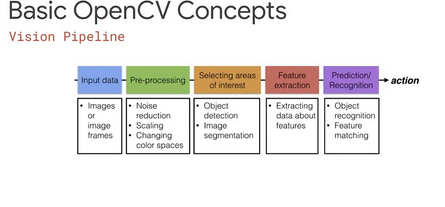
\includegraphics[width=0.8\textwidth]{convolution.png}
        \caption{Minh họa các phép toán tích chập và gộp.}
        \label{fig:cnn_ops}
    \end{figure}
    Các kiến trúc CNN nổi bật bao gồm \textbf{ResNet} \cite{he2016deep} (sử dụng kết nối dư để giải quyết vấn đề gradient vanishing) và các mô hình phát hiện đối tượng như \textbf{Faster R-CNN} \cite{ren2015faster} (phương pháp hai giai đoạn) và \textbf{YOLO} \cite{redmon2016you} (phương pháp một giai đoạn, cực kỳ nhanh).

    \item \textbf{Mô hình dựa trên Transformer}:
    Gần đây, các mô hình dựa trên Transformer đã đạt được hiệu suất ấn tượng trong thị giác. \textbf{Vision Transformer (ViT)} \cite{dosovitskiy2021image} chia hình ảnh thành các miếng vá (patches) và xử lý chúng như một chuỗi token, sử dụng cơ chế tự chú ý (self-attention) để tính toán mối quan hệ giữa các miếng vá:
    \begin{equation}
    \text{Attention}(Q, K, V) = \text{softmax}\left(\frac{QK^T}{\sqrt{d_k}}\right)V
    \label{eq:attention_full}
    \end{equation}
    \begin{figure}[h]
        \centering
        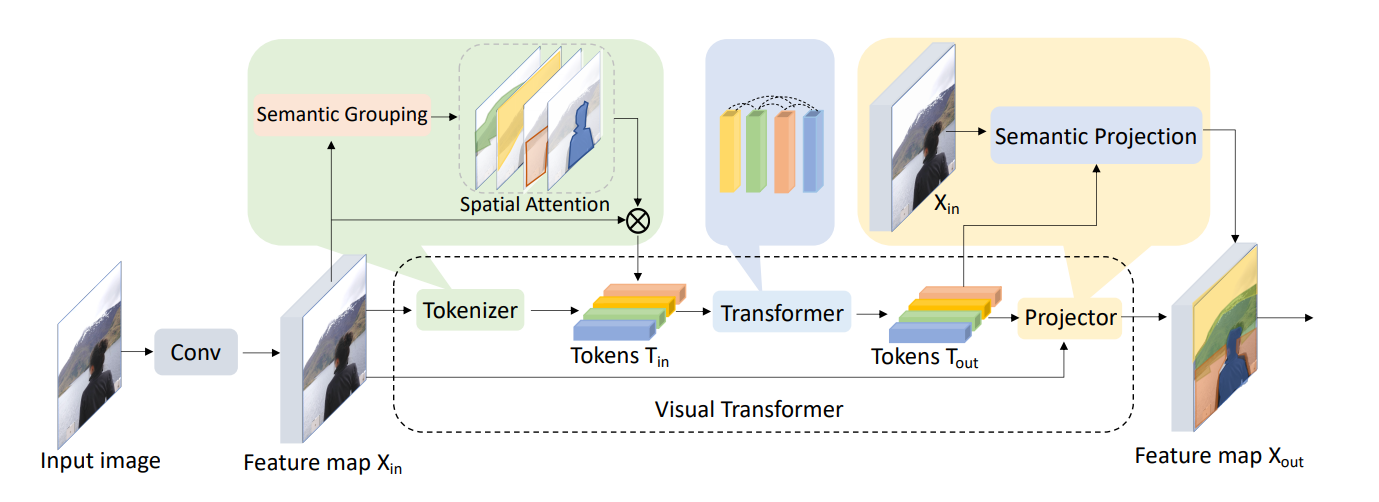
\includegraphics[width=0.9\textwidth]{visual_transformer.png}
        \caption{Sơ đồ kiến trúc Vision Transformer (ViT).}
        \label{fig:vit_arch}
    \end{figure}
\end{itemize}

\subsubsection{Các tập dữ liệu và metrics đánh giá}
Đánh giá hiệu suất của các mô hình CV dựa trên các tập dữ liệu chuẩn mực và metrics khách quan:
\begin{itemize}
    \item \textbf{Tập dữ liệu}: COCO \cite{lin2014microsoft}, ImageNet \cite{deng2009imagenet}, Pascal VOC \cite{everingham2015pascal}, Cityscapes \cite{cordts2016cityscapes}.
    \item \textbf{Metrics}:
    \begin{itemize}
        \item \textbf{IoU (Intersection over Union)}: Đo lường độ trùng lặp giữa hộp giới hạn dự đoán và thực tế.
        \item \textbf{mAP (Mean Average Precision)}: Metric tiêu chuẩn cho phát hiện đối tượng, tính trung bình của độ chính xác trung bình (AP) trên tất cả các lớp.
        \item \textbf{F1-score}: Trung bình điều hòa của độ chính xác (precision) và độ phủ (recall), được sử dụng rộng rãi trong các bài toán phân loại.
    \end{itemize}
\end{itemize}

\subsection{Ước lượng Dáng người: Các phương pháp và ứng dụng}
Ước lượng Dáng người (HPE) là tác vụ chuyên biệt nhằm xác định vị trí các khớp xương (keypoints) của cơ thể người. Lĩnh vực này đã tiến bộ vượt bậc, từ các phương pháp thủ công sang các mô hình học sâu mạnh mẽ.

\subsubsection{Phân loại các phương pháp}
Các phương pháp HPE hiện đại thường được phân loại dựa trên cách chúng xử lý bài toán đa người:
\begin{itemize}
    \item \textbf{Phương pháp từ trên xuống (Top-Down)}: Phương pháp này áp dụng hai bước tuần tự. Đầu tiên, một bộ phát hiện đối tượng sẽ tìm tất cả các cá nhân trong hình ảnh. Sau đó, một mô hình ước lượng dáng người cho một người sẽ được chạy trên từng bounding box đã phát hiện. Phương pháp này có độ chính xác cao nhưng có thể chậm khi số lượng người lớn. Các ví dụ nổi bật bao gồm \textbf{AlphaPose} \cite{fang2017rmpe}.
    \item \textbf{Phương pháp từ dưới lên (Bottom-Up)}: Phương pháp này hiệu quả hơn cho các cảnh đông người. Nó phát hiện tất cả keypoints trong khung hình trước, sau đó sử dụng một thuật toán để nhóm các keypoints này lại với nhau, tạo thành các dáng người hoàn chỉnh. \textbf{OpenPose} \cite{cao2017realtime} là một ví dụ kinh điển, sử dụng Part Affinity Fields (PAFs) để mã hóa mối quan hệ giữa các khớp.
\end{itemize}
\begin{figure}[h]
    \centering
    \begin{subfigure}[b]{0.45\textwidth}
        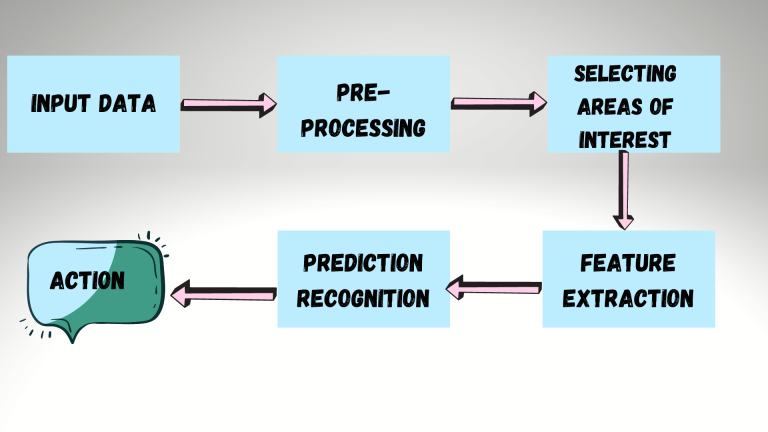
\includegraphics[width=\textwidth]{top_down.png}
        \caption{Quy trình từ trên xuống (Top-Down).}
    \end{subfigure}
    \hfill
    \begin{subfigure}[b]{0.45\textwidth}
        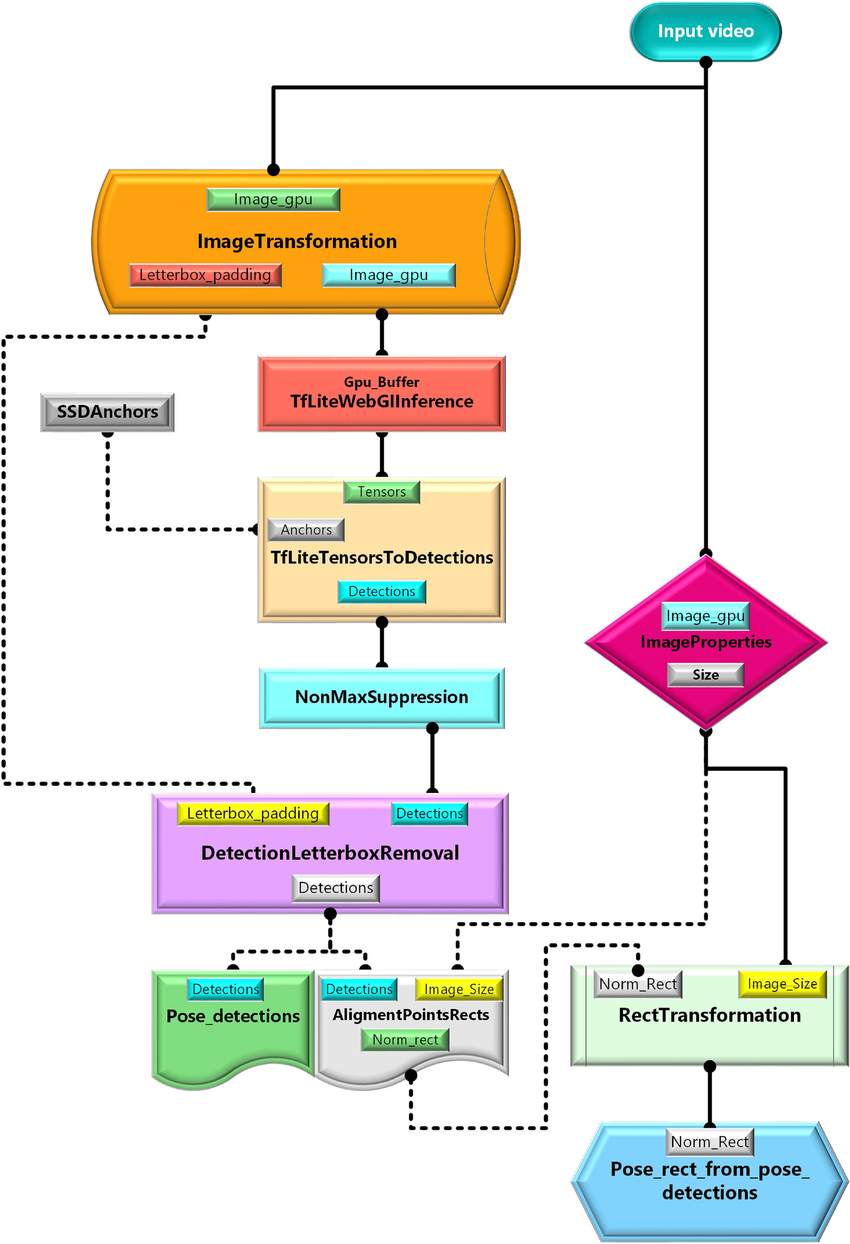
\includegraphics[width=\textwidth]{bottom_up.png}
        \caption{Quy trình từ dưới lên (Bottom-Up).}
    \end{subfigure}
    \caption{So sánh hai quy trình chính trong ước lượng dáng người đa người.}
\end{figure}
Kiến trúc mạng như \textbf{HRNet} (High-Resolution Network) \cite{sun2019deep} đã được thiết kế đặc biệt để giải quyết các vấn đề về độ phân giải, duy trì biểu diễn đặc trưng ở độ phân giải cao trong suốt quá trình xử lý, giúp định vị keypoint chính xác hơn.

\subsubsection{Datasets và Metrics đánh giá trong HPE}
Đánh giá mô hình HPE yêu cầu các tập dữ liệu và metrics chuyên biệt:
\begin{itemize}
    \item \textbf{Datasets}:
    \begin{itemize}
        \item \textbf{COCO Keypoints} \cite{lin2014microsoft}: Mở rộng của COCO, là tiêu chuẩn vàng cho ước lượng dáng người 2D với 17 keypoints.
        \item \textbf{MPII Human Pose} \cite{andriluka20142d}: Một tập dữ liệu nổi tiếng khác với 16 keypoints và các chú thích chi tiết về hoạt động.
        \item \textbf{Human3.6M} \cite{ionescu2014human36m}: Tập dữ liệu quy mô lớn cung cấp thông tin keypoint 3D, rất quan trọng cho nghiên cứu 3D HPE.
    \end{itemize}
    \begin{table}[h]
        \centering
        \caption{Bảng so sánh các Dataset chính trong Ước lượng Dáng người.}
        \label{tab:hpe_datasets}
        \begin{tabular}{lccc}
            \toprule
            \textbf{Dataset} & \textbf{Số lượng ảnh} & \textbf{Số Keypoints} & \textbf{Loại chú thích} \\
            \midrule
            COCO Keypoints & $\sim 200$k & $17$ & 2D Keypoints \\
            MPII Human Pose & $\sim 25$k & $16$ & 2D Keypoints \\
            Human3.6M & $\sim 3.6$M & $17$ & 3D Keypoints \\
            \bottomrule
        \end{tabular}
    \end{table}
    \item \textbf{Metrics}:
    \begin{itemize}
        \item \textbf{PCK (Percentage of Correct Keypoints)}: Tỷ lệ các keypoint được dự đoán nằm trong một khoảng cách nhất định so với ground truth.
        \item \textbf{OKS (Object Keypoint Similarity)}: Metric chính trong COCO Keypoints, đánh giá sự tương đồng giữa keypoint dự đoán và ground truth, có tính đến kích thước đối tượng và độ quan trọng của từng keypoint.
        \begin{equation}
        OKS = \frac{\sum_i \exp\left(-\frac{d_i^2}{2s^2k_i^2}\right) \cdot \delta(v_i > 0)}{\sum_i \delta(v_i > 0)}
        \label{eq:oks}
        \end{equation}
        trong đó $d_i$ là khoảng cách Euclidean, $s$ là diện tích đối tượng và $k_i$ là hằng số trọng số của keypoint $i$.
    \end{itemize}
\end{itemize}

\section{Phân tích chuyên sâu MediaPipe Pose Estimation và ứng dụng}

Mục này đi sâu vào phân tích \textbf{MediaPipe Pose Estimation} của Google, một giải pháp tiên tiến được tối ưu hóa cho các ứng dụng thời gian thực trên đa nền tảng.

\subsection{Kiến trúc và Pipeline của MediaPipe}
Pipeline của MediaPipe được xây dựng trên kiến trúc \textbf{graph-based processing}, cho phép xử lý dữ liệu theo một đồ thị linh hoạt. Nó bao gồm ba mô hình học sâu chính, hoạt động tuần tự để đạt được độ chính xác và hiệu suất tối ưu:
\begin{enumerate}
    \item \textbf{Mô hình Phát hiện Tư thế (Pose Detection Model)}: Đây là giai đoạn đầu tiên, sử dụng một kiến trúc CNN nhẹ để xác định vị trí cơ thể người trong khung hình và tạo ra một hộp giới hạn (bounding box).
    \item \textbf{Mô hình Điểm mốc Tư thế (Pose Landmark Model - BlazePose)}: Mô hình cốt lõi. Sau khi nhận được bounding box, nó dự đoán vị trí chi tiết của 33 keypoints 3D trên cơ thể. \textbf{BlazePose} sử dụng các khối xây dựng hiệu quả như Depthwise Separable Convolutions để giảm số lượng tham số, giúp mô hình nhỏ gọn và chạy nhanh.
    \item \textbf{Mô hình Theo dõi Tư thế (Pose Tracking Model)}: Để tối ưu hóa tốc độ, mô hình này sử dụng các thông tin từ khung hình trước đó để dự đoán ROI cho khung hình hiện tại. Điều này giảm đáng kể chi phí tính toán so với việc chạy lại mô hình phát hiện đầy đủ ở mỗi khung hình.
\end{enumerate}
\begin{figure}[h]
    \centering
    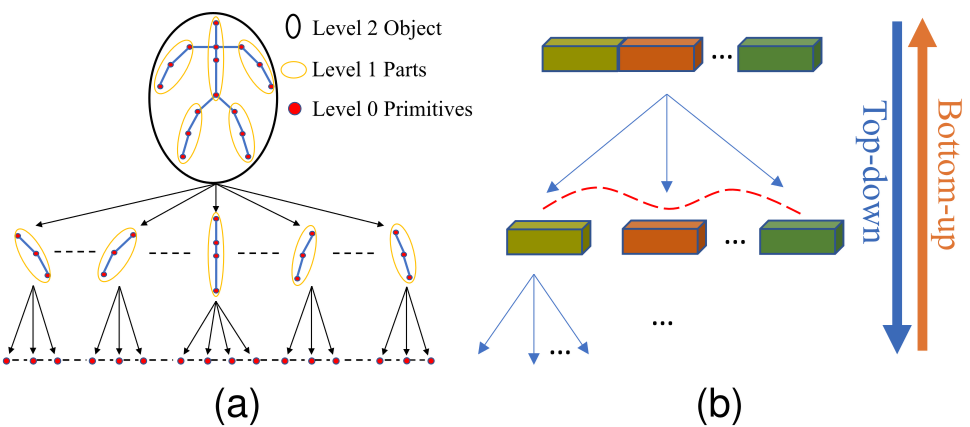
\includegraphics[width=0.9\textwidth]{quy_trinh_ba_mo_hinh.png}
    \caption{Sơ đồ quy trình xử lý ba mô hình của MediaPipe Pose Estimation.}
    \label{fig:mediapipe_pipeline}
\end{figure}

\subsection{Thuật toán tiền xử lý và hậu xử lý}
Để tối ưu hóa hiệu suất, MediaPipe tích hợp các thuật toán xử lý bổ sung:
\begin{itemize}
    \item \textbf{Bộ lọc làm mịn (Smoothing Filter)}: Sau khi các keypoint được ước tính, một bộ lọc làm mịn temporal như \textbf{One Euro Filter} được áp dụng để giảm nhiễu và đảm bảo sự mượt mà của các keypoints theo thời gian.
    \item \textbf{Tinh chỉnh điểm mốc (Landmark Refinement)}: Một số phiên bản phức tạp hơn có thể bao gồm bước tinh chỉnh cuối cùng để điều chỉnh vị trí keypoints dựa trên các ràng buộc về hình học hoặc giải phẫu học.
\end{itemize}

\subsection{Ứng dụng thực tế: Xây dựng thuật toán phát hiện té ngã}
Dữ liệu keypoint 3D từ MediaPipe cung cấp thông tin phong phú để xây dựng các thuật toán nhận dạng hành vi phức tạp, ví dụ như phát hiện té ngã. Thuật toán có thể hoạt động dựa trên ba giai đoạn chính:
\begin{enumerate}
    \item \textbf{Phát hiện cú ngã đột ngột}: Xác định một cú ngã bằng cách theo dõi tốc độ thay đổi vị trí của các keypoint quan trọng như đầu và hông.
    \item \textbf{Phân tích tư thế sau cú ngã}: Kiểm tra xem người dùng có đang ở tư thế nằm ngang hay không, dựa trên tỷ lệ khung hình (aspect ratio) của cơ thể.
    \item \textbf{Xác minh trạng thái bất động}: Sử dụng một bộ đếm thời gian. Nếu người dùng không di chuyển trong một khoảng thời gian nhất định sau khi đáp ứng hai điều kiện trên, hệ thống sẽ kích hoạt cảnh báo.
\end{enumerate}
\begin{figure}[h]
    \centering
    \begin{tikzpicture}[node distance=2cm, auto, thick, font=\sffamily, startstop/.style={rectangle, rounded corners, draw, fill=blue!20, minimum width=3cm, minimum height=1cm, align=center}, process/.style={rectangle, draw, fill=green!20, minimum width=3cm, minimum height=1cm, align=center}, decision/.style={diamond, draw, fill=orange!20, minimum width=3cm, aspect=1.5, align=center, inner sep=0pt}]
        \node (start) [startstop] {Bắt đầu};
        \node (proc1) [process, below of=start] {Giai đoạn 1:\\Phát hiện cú ngã đột ngột};
        \node (proc2) [process, below of=proc1] {Giai đoạn 2:\\Phân tích tư thế};
        \node (proc3) [process, below of=proc2] {Giai đoạn 3:\\Xác minh trạng thái bất động};
        \node (decision) [decision, below of=proc3, yshift=-1cm] {Té ngã được\\xác nhận?};
        \node (stop1) [startstop, right of=decision, xshift=3cm] {Kích hoạt cảnh báo};
        \node (stop2) [startstop, below of=decision, yshift=-1cm] {Kết thúc};

        \draw[->] (start) -- (proc1);
        \draw[->] (proc1) -- (proc2);
        \draw[->] (proc2) -- (proc3);
        \draw[->] (proc3) -- (decision);
        \draw[->] (decision) -- node[above] {Có} (stop1);
        \draw[->] (decision) -- node[left] {Không} (stop2);
    \end{tikzpicture}
    \caption{Sơ đồ logic của thuật toán phát hiện té ngã dựa trên dữ liệu keypoint.}
    \label{fig:fall_detection}
\end{figure}

\subsection{So sánh và Thảo luận mở rộng}
\subsubsection{So sánh các giải pháp}
Việc so sánh MediaPipe với các giải pháp khác như \textbf{OpenPose}, \textbf{MoveNet}, và \textbf{YOLOv7-Pose} cho thấy MediaPipe đạt được sự cân bằng tối ưu giữa độ chính xác và tốc độ suy luận, đặc biệt là trên các thiết bị nhúng. Trong khi OpenPose nổi bật về độ chính xác, MediaPipe và MoveNet vượt trội hơn về tốc độ và khả năng triển khai trên thiết bị có tài nguyên hạn chế.
\begin{table}[h]
    \centering
    \caption{Bảng so sánh chi tiết giữa các giải pháp Pose Estimation hàng đầu.}
    \label{tab:comparison_pose_detailed}
    \begin{tabular}{|l|l|l|l|l|}
        \hline
        \textbf{Tiêu chí} & \textbf{MediaPipe Pose} & \textbf{YOLOv7-Pose} & \textbf{OpenPose} & \textbf{MoveNet} \\
        \hline
        \textbf{Số keypoints} & 33 (3D) & 17 (2D) & 25 (2D) & 17 (2D) \\
        \hline
        \textbf{Kích thước mô hình} & Detection: 815K\newline Landmarks: 3.37M & $\sim$37M params & $\sim$200M params & Lightning: 1.5M\newline Thunder: 7M \\
        \hline
        \textbf{Độ chính xác (mAP)} & 0.65-0.75 & 0.68-0.78 & 0.70-0.80 & 0.60-0.72 \\
        \hline
        \textbf{FPS (RTX 3080)} & 60-100 & 45-80 & 25-45 & 80-120 \\
        \hline
        \textbf{FPS (CPU i7)} & 25-40 & 15-25 & 8-15 & 30-60 \\
        \hline
        \textbf{Ước tính 3D} & Có & Không & Không & Không \\
        \hline
        \textbf{Tương thích} & Python, C++\newline Web, Mobile & Python, C++ & Python, C++\newline CUDA & Python, C++\newline Web, Mobile \\
        \hline
    \end{tabular}
\end{table}

\subsubsection{Các thách thức và hướng đi tương lai}
Mặc dù đã có những tiến bộ đáng kể, ước lượng dáng người vẫn đối mặt với các thách thức lớn như xử lý \textbf{che khuất nghiêm trọng (occlusion)}, các biến thể về ánh sáng và góc quay, và tối ưu hóa cho môi trường đa người. Tương lai của lĩnh vực này sẽ tập trung vào việc phát triển các mô hình mạnh mẽ hơn, hiệu quả hơn và có khả năng suy luận trong thời gian thực trên các thiết bị phân tán.

